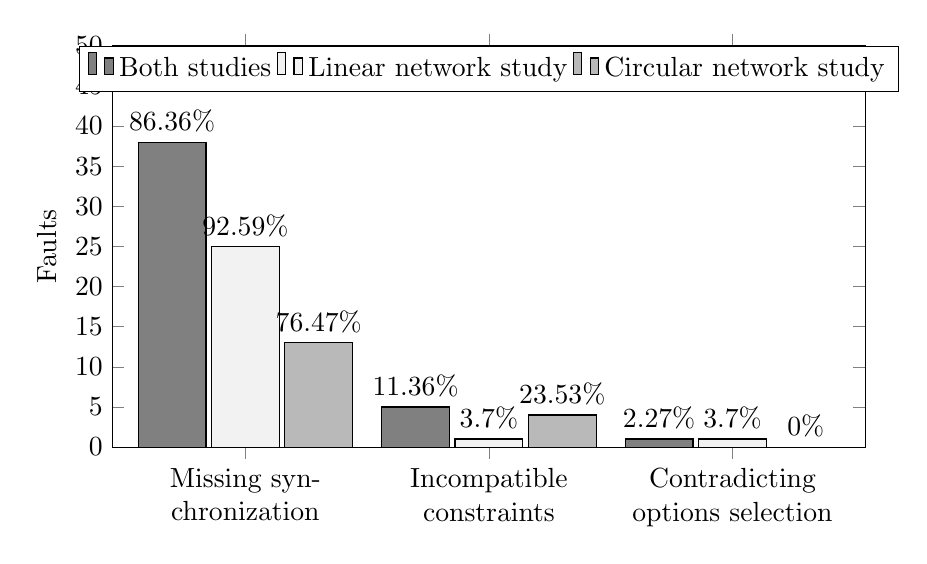
\begin{tikzpicture}
    \begin{axis}[
        ybar,
        bar width=2.45em,
        x=8.8em,
        height=19em,
        legend style={at={(0.5,1)},anchor=north,legend columns=-1},
        ylabel={Faults},
        symbolic x coords={Missing synchronization, Incompatible constraints, Contradicting options selection},
        xticklabel style={text width=8em, align=center},
        xtick=data,
        ytick distance=5,
        ymin=0,
        ymax=50,
        enlarge x limits={abs=4.8em},
        nodes near coords align={vertical},
    ]
    \addplot[fill=gray,
        point meta={y*100/44}, % 44 Mistakes in total, calculate percentage
        nodes near coords={\pgfmathprintnumber\pgfplotspointmeta\%},
        ] table[x=Mistake Type, y=occurrences, col sep=comma] {
            Mistake Type,                       occurrences
            Missing synchronization,            38
            Incompatible constraints,           5
            Contradicting options selection,    1
        };
    \addplot[fill=gray!10,
        point meta={y*100/27}, % 27 Mistakes in total, calculate percentage
        nodes near coords={\pgfmathprintnumber\pgfplotspointmeta\%},
        ] table[x=Mistake Type, y=occurrences, col sep=comma] {
            Mistake Type,                       occurrences
            Missing synchronization,            25
            Incompatible constraints,           1
            Contradicting options selection,    1
        };
    \addplot[fill=gray!55,
        point meta={y*100/17}, % 17 Mistakes in total, calculate percentage
        nodes near coords={\pgfmathprintnumber\pgfplotspointmeta\%},
        ] table[x=Mistake Type, y=occurrences, col sep=comma] {
            Mistake Type,                       occurrences
            Missing synchronization,            13
            Incompatible constraints,           4
            Contradicting options selection,    0
        };
        \legend{Both studies, Linear network study, Circular network study}
    \end{axis}
\end{tikzpicture}